\documentclass[12pt,titlepage,a4paper]{article}
%\documentclass[a4paper,fontsize=13pt]{scrartcl}

\usepackage{vntex}
%\usepackage{helvet} %set font Helvetica

%\usepackage{times} %set font Times New Roman
%\renewcommand{\familydefault}{\sfdefault} %set font Sans Serif

%\usepackage[english,vietnam]{babel}
%\usepackage[utf8]{inputenc}

\usepackage[utf8]{inputenc}
%\usepackage[francais]{babel}
\usepackage{a4wide,amssymb,epsfig,latexsym,array,hhline,fancyhdr}
\usepackage{framed}    % đóng khung đoạn văn
\usepackage{amsmath}
\usepackage{amsthm}
\usepackage{multicol,longtable,amscd}
\usepackage{diagbox}%Make diagonal lines in tables
\usepackage{booktabs}
\usepackage{alltt}

\usepackage{lastpage}
\usepackage[lined,boxed,commentsnumbered]{algorithm2e}
\usepackage{enumerate}
\usepackage{xcolor}
\usepackage{graphicx}							% Standard graphics package
\usepackage{array}
\usepackage{tabularx, caption}
\usepackage{multirow}
\usepackage{framed}    % đóng khung đoạn văn
\usepackage{verbatim}  % định dạng text
\usepackage{multicol}
\usepackage{rotating}
\usepackage{graphics}
\usepackage[left=2cm,right=2cm,top=2cm,bottom=3cm]{geometry}

\usepackage{setspace}
%\singlespacing
%\onehalfspacing
%\doublespacing
%\setstretch{1.5}


\usepackage{epsfig}
\usepackage{tikz}
\usetikzlibrary{calc}
\newcommand\HRule{\rule{\textwidth}{1pt}}
\usetikzlibrary{arrows,snakes,backgrounds}
\usepackage[unicode]{hyperref}
\hypersetup{urlcolor=blue,linkcolor=black,citecolor=black,colorlinks=true} 
%\usepackage{pstcol} 								% PSTricks with the standard color package

\usepackage{a4wide,amssymb,epsfig,latexsym,array,hhline,fancyhdr}

\usepackage[makeroom]{cancel}
\usepackage{amsmath}
\usepackage{amsthm}
\usepackage{multicol,longtable,amscd}
\usepackage{diagbox}%Make diagonal lines in tables
\usepackage{booktabs}
\usepackage{alltt}
\usepackage[framemethod=tikz]{mdframed}% For highlighting paragraph backgrounds
\usepackage{caption,subcaption}
\usepackage{arydshln}
\usepackage{tabularx} % in the preamble

\setlength\dashlinedash{1.5pt}
\setlength\dashlinegap{4.5pt}
\setlength\arrayrulewidth{0.2pt}

\usepackage{textcomp}
\usepackage{listings}
\usepackage{listingsutf8}
% Typesetting Listings
\usepackage{xcolor}
\usepackage{color}
\definecolor{listinggray}{gray}{0.9}
\definecolor{lbcolor}{rgb}{0.9,0.9,0.9}
\definecolor{Darkgreen}{rgb}{0.1,0.6,0.1}

\lstset{
	backgroundcolor=\color{lbcolor},
	tabsize=4,    
	%   rulecolor=,
	language=[GNU]C++,
	basicstyle=\scriptsize,
	upquote=true,
	aboveskip={1.5\baselineskip},
	columns=fixed,
	showstringspaces=false,
	extendedchars=false,
	breaklines=true,
	prebreak = \raisebox{0ex}[0ex][0ex]{\ensuremath{\hookleftarrow}},
	frame=single,
	numbers=left,
	showtabs=false,
	showspaces=false,
	showstringspaces=false,
	identifierstyle=\ttfamily,
	keywordstyle=\color[rgb]{0,0,1},
	commentstyle=\color[rgb]{0.026,0.112,0.095},
	stringstyle=\color[rgb]{0.627,0.126,0.941},
	numberstyle=\color[rgb]{0.205, 0.142, 0.73},
	%        \lstdefinestyle{C++}{language=C++,style=numbers}’.
}
\lstset{
	backgroundcolor=\color{lbcolor},
	tabsize=4,
	language=C++,
	captionpos=b,
	tabsize=3,
	frame=lines,
	numbers=left,
	numberstyle=\tiny,
	numbersep=5pt,
	breaklines=true,
	showstringspaces=false,
	basicstyle=\footnotesize,
	%  identifierstyle=\color{magenta},
	keywordstyle=\color[rgb]{0,0,1},
	commentstyle=\color{Darkgreen},
	stringstyle=\color{red}
}

\usepackage{lastpage}
\usepackage[lined,boxed,commentsnumbered]{algorithm2e}
\usepackage{enumerate}
\usepackage{color}
\usepackage{graphicx}							% Standard graphics package
\usepackage{array}
\usepackage{tabularx, caption}
\usepackage{multirow}
\usepackage{multicol}
\usepackage{rotating}
\usepackage{graphics}
\usepackage{geometry}
\usepackage{setspace}
\usepackage{epsfig}
\usepackage{tikz}
\usetikzlibrary{arrows,snakes,backgrounds}
\usepackage[unicode]{hyperref}
\hypersetup{urlcolor=blue,linkcolor=black,citecolor=black,colorlinks=true} 
%\usepackage{pstcol} 								% PSTricks with the standard color package
\usepackage{verbatim}

 


%\usepackage{fancyhdr}
\setlength{\headheight}{40pt}
\pagestyle{fancy}
\fancyhead{} % clear all header fields
\fancyhead[L]{
 \begin{tabular}{rl}
	\begin{tabular}{l}
		\textbf{\bf \ttfamily Trường ĐHBK - Khoa KH và KT Máy tính}\\
	\end{tabular} 	
 \end{tabular}
}
\fancyhead[R]{
	\begin{tabular}{l}
		\tiny \bf \\
		\tiny \bf 
	\end{tabular}  }
\fancyfoot{} % clear all footer fields
\fancyfoot[L]{\scriptsize \ttfamily Phát triển ứng dụng Internet of Things} %Nội dung của footer ở đây
\fancyfoot[R]{\scriptsize \ttfamily Trang  {\thepage}/\pageref{LastPage}} % page number
\renewcommand{\headrulewidth}{1pt}
\renewcommand{\footrulewidth}{1pt}
%%%
\setcounter{secnumdepth}{4}
\setcounter{tocdepth}{3}
\makeatletter
\newcounter {subsubsubsection}[subsubsection]
\renewcommand\thesubsubsubsection{\thesubsubsection .\@alph\c@subsubsubsection}
\newcommand\subsubsubsection{\@startsection{subsubsubsection}{4}{\z@}%
                                     {-3.25ex\@plus -1ex \@minus -.2ex}%
                                     {1.5ex \@plus .2ex}%
                                     {\normalfont\normalsize\bfseries}}
\newcommand*\l@subsubsubsection{\@dottedtocline{3}{10.0em}{4.1em}}
\newcommand*{\subsubsubsectionmark}[1]{}
\makeatother
\everymath{\color{black}}%make in-line maths symbols blue to read/check easily
\sloppy
\captionsetup[figure]{labelfont={small,bf},textfont={small,it},belowskip=-1pt,aboveskip=-9pt}
%space remove between caption, figure, and text
\captionsetup[table]{labelfont={small,bf},textfont={small,it},belowskip=-1pt,aboveskip=7pt}
\setlength{\floatsep}{5pt plus 2pt minus 2pt}
\setlength{\textfloatsep}{5pt plus 2pt minus 2pt}
\setlength{\intextsep}{10pt plus 2pt minus 2pt}

%%%%%%%%%%%%%%%%%%%%%%%%%%%%%%%%%%%%%%%%%%%%%%%%%%%%%%
% Initilization done. Now document starts.


\begin{document}
\begin{titlepage}
\begin{tikzpicture}[remember picture, overlay]
  \draw[line width = 2pt,color=blue] ($(current page.north west) + (2.7cm,-2.7cm)$) rectangle ($(current page.south east) + (-2.7cm,2.7cm)$);
   \draw[line width = 1pt,color=green] ($(current page.north west) + (2.6cm,-2.6cm)$) rectangle ($(current page.south east) + (-2.6cm,2.6cm)$);
\end{tikzpicture}
\vspace{0cm}
\begin{center}
Trường Đại học Bách Khoa - ĐHQG HCM\\
\textbf{Khoa Khoa học và Kỹ thuật Máy tính } \\
- - - - - - - - - - - -
\end{center}


\vspace{1cm}
\begin{figure}[h!]
\begin{center}
\includegraphics[width=3.6cm]{Figures/hcmut.png}
\end{center}
\end{figure}
\vspace{1cm}



\begin{center}
\begin{tabular}{c}
\multicolumn{1}{c}{\textbf{{\large Phát triển ứng dụng Internet of Things}}}\\
~~\\ %% Tên môn học ở đây
\hline
\\
\multicolumn{1}{c}{\textbf{{\Large Weather Station}}}\\
\\
\textbf{{\Large Hệ thống theo dõi môi trường}} \\ %% Tên đề tài line 1
\textbf{{\Large và điều khiển đèn ngủ thông minh }} %% Tên đề tài line 2 %% short description
\\[0.3cm]
\hline
\end{tabular}
\end{center}

\begin{table}[h]
\begin{tabular}{ll}
\hspace{2.75cm} GVHD: & TS. Lê Trọng Nhân \\
& TS. Nguyễn Trần Hữu Nguyên \\
\end{tabular}
\end{table}
%\vspace{0.5cm}
\begin{table}[h]
\begin{tabular}{lll}
\hspace{2.75cm} Sinh viên: & Hoàng Nguyễn Minh Đức & 1610755\\
& Thái Thị Thanh Linh & 1611830 \\
& Lê Đức Thịnh & 1613346 \\
& Lê Minh Thịnh & 1513249
\end{tabular}
\end{table}

\vspace{3.2cm}
\begin{center}
{\footnotesize TP. Hồ Chí Minh, tháng 12 2018}
\end{center}
\end{titlepage}

%Mục lục
\newpage
\thispagestyle{empty}
\tableofcontents

%Danh sách bảng
%\newpage
%\thispagestyle{empty}
%\listoftables

%Danh sách hình
%\newpage
%\thispagestyle{empty}
%\listoffigures


%%%%%%%%%%%%%%%%%%%%%%%%%%%
% Page 1
\newpage
\section{Khái quát đề tài}
\subsection{Giới thiệu}
\begin{itemize}
\item Hiện thực một hệ thống thu thập dữ liệu môi trường từ các cảm biến, sau đó các dữ liệu này sẽ được các nodes (ESP8266) gửi đến server (Raspberry Pi 3 B). Server sẽ có nhiệm vụ lưu trữ các dữ liệu này trên database (Firebase). Từ cơ sở dữ liệu này sẽ được truy cập để hiển thị đến người dùng thông qua ứng dụng di động và website.
\item Trong số các dữ liệu thu thập được, các số liệu về cường độ ánh sáng sẽ được sử dụng để tự động bật - tắt thiết bị đèn.
\end{itemize}
\subsection{Phần cứng sử dụng}
\subsubsection{NodeMCU ESP8266}
NodeMCU ESP8266 được phát triển dựa trên Chip WiFi ESP8266EX tích hợp bên trong module ESP-12E, cho phép kết nối WiFi một cách đơn giản. Ngoài ra, module còn hỗ trợ giao tiếp với PC thông qua Micro USB phổ biến. 
\begin{itemize}
\item Số lượng: 3.
\item Chức năng: Hoạt động như các socket client, thu thập dữ liệu từ cảm biến và gửi đến socket server. Ngoài ra còn hiển thị các thông tin thu thập được về môi trường lên màn hình LCD 16x2 và điều khiển bật - tắt đèn một cách tự động.
\end{itemize}
\subsubsection{Raspberry Pi 3 B}
Raspberry Pi 3 B là một máy tính nhúng có kích thước nhỏ gọn với các thành phần cơ bản như CPU, RAM, kết nối WiFi và cổng USB. Pi 3 có thể được sử dụng vào nhiều mục đích khác nhau vì tính đa dụng cũng như cộng đồng hỗ trợ rộng lớn và mạnh mẽ.
\begin{itemize}
\item Số lượng: 1.
\item Chức năng: Hoạt động như một local socket server, tiếp nhận dữ liệu từ các client và gửi lên online server.
\end{itemize}
\subsubsection{Các module cảm biến}
\begin{enumerate}
\item DHT11:
\begin{itemize}
\item Số lượng: 1.
\item Chức năng: *Linh's section*
\end{itemize}
\item *name of light module here*:
\begin{itemize}
\item Số lượng: 1.
\item Chức năng: *Linh's section*
\end{itemize}
\end{enumerate}
\subsubsection{Màn hình LCD 16x2}
\begin{itemize}
\item Số lượng: 1.
\item Chức năng: Hiển thị thông tin về môi trường xung quanh thông qua dữ liệu lấy từ server và trạng thái bật - tắt của đèn.
\end{itemize}
\subsubsection{Những linh kiện khác}
Ngoài các phần cứng kể trên, đề tài còn sử dụng các linh kiện khác như: Cáp Micro USB, dây dẫn, Breadboard và đèn ngủ.

\subsection{Phần mềm sử dụng}
\subsubsection{Android Studio}
Android Studio là IDE (môi trường phát triển tích hợp) chính thức cho nền tảng Android, được phát triển bởi Google. Ngôn ngữ lập trình được sử dụng để phát triển trong đề tài là Java trên nền tảng Android Things, hỗ trợ cho board Raspberry Pi 3 B.
\subsubsection{Arduino IDE}
Tương tự như Android Studio, Arduino IDE là môi trường phát triển chính thức dành cho nền tảng Arduino. Arduino hỗ trợ nhiều board khác nhau, một trong số đó là NodeMCU ESP8266.
\subsubsection{Visual Studio Code}
Visual Studio Code là một trình biên tập mã được phát triển bởi Microsoft, cung cấp cho lập trình viên nhiều tùy chỉnh khác nhau.
\\
Trong đề tài này, Visual Studio Code được sử dụng như một công cụ soạn thảo để phát triển mã nguồn của server (Node JS - Java Script) và ứng dụng di động (React Native - Java Script).
\subsubsection{Adobe Muse}
*Thinh's section*
\subsubsection{SocketTest}
*description goes here*

\newpage
\section{Tổng quan hệ thống}
\subsection{Sơ đồ khối}
\subsection{•}

\newpage
\section{Hiện thực hệ thống}
\subsection{Socket clients}
*Linh's section*
\subsection{Socket server}
*Duc's section*
\subsection{Module hiển thị và điều khiển}
*Duc's section*
\subsection{Online server}
*Duc's section*
\subsection{Ứng dụng di động}
*A Thinh's section*
\subsection{Website}
*Thinh's section*

\newpage
%%%%%%%%%%%%%%%%%%%%%%%%%%%%%%%%%%%%%%%%%%%%%%%%%%%%%%%%%%%%%%%% Thinh
\section{App}

\subsection{UI}
\subsubsection{Web App}
\begin{figure}[h]
    \centering
    \includegraphics[width=40mm]{Figures/wea_mobile.png}
    \includegraphics[width=32mm]{Figures/set_mobile.png}
    \caption{web Weather Station trên di động}
    \label{wea_mobile}
\end{figure}

\begin{figure}[h]
    \centering
    \includegraphics[width=100mm]{Figures/wea_wide.png}\\
    \includegraphics[width=100mm]{Figures/sett_wide.png}
    \caption{web Weather Station trên máy tính}
    \label{wea_mobile}
\end{figure}
\newpage
Các giao diện chính của Weather Station trên web app gồm có Weather, Widgets và Settings.\\
\textbf{Weather: } Ở đây các thông số về nhiệt độ, độ ẩm, thời tiết sẽ được cập nhật từ thông số cuối cùng được ghi trên Server.
Hình ảnh nền phía sau sẽ thay đổi dựa trên thời gian người dùng truy cập vào trang web.\\
\textbf{Widgets: } \(Trong quá trình phát triển\) Khi liên kết với các thiết bị IoT khác, có thể sử dụng các số liệu từ cảm biến ghi lại được và tự động hóa các hoạt động khác như điều khiển đèn, điều khiển quạt, máy điều hòa, etc.\\
\textbf{Settings: } Dùng điều chỉnh hiển thị độ C và độ F ở màn hình Weather và tần số cập nhật số liệu, đồng thời hiện các thông tin chính về project cũng như nhóm thực hiện.


\subsection{Code}
%%%%%%%%%%%%%%%%%%%%%%%%%%%%%%%%%%%%%%%%%%%%%%%%%%%%%%%%%%%%%%%%%%%%%

\newpage
%\renewcommand{\refname}{Tài liệu tham khảo}
\begin{thebibliography}{39}
	\bibitem{Hennessy:Patterson:2007}
		John L.Hennessy and David A.Patterson, 
		\textit{Computer Architecture A Quantitative Approach}, Morgan Kaufmann Publisher, 2007, pp. 8-12
	\bibitem{Stallings:2010}
		William Stallings,
		\textit{Computer Organization and Architecture Designing for Performance ($8^{th} ed.$)}, Pearson Prentice Hal, 2010. pp. 18-19, 496, 517.
	\bibitem{YiGao:2010}
		Gao, Shilang Tang, Zhangli Ding,
		\textit{Comparison between CISC and RISC}, 2000
\end{thebibliography}

\end{document}

